\documentclass{article}
\usepackage{amsmath}

\usepackage{graphicx}

\usepackage{listings}
\usepackage{color}
\definecolor{dkgreen}{rgb}{0,0.6,0}
\definecolor{gray}{rgb}{0.5,0.5,0.5}
\definecolor{mauve}{rgb}{0.58,0,0.82}
\lstset{frame=tb,
  language=R,
  aboveskip=3mm,
  belowskip=3mm,
  showstringspaces=false,
  columns=flexible,
  basicstyle={\small\ttfamily},
  numbers=none,
  numberstyle=\tiny\color{gray},
  keywordstyle=\color{blue},
  commentstyle=\color{dkgreen},
  stringstyle=\color{mauve},
  breaklines=false,
  breakatwhitespace=true,
  tabsize=3
}

\title{SDS385 Fall '16: Statistical Models For Big Data\\Exercises 03 - Quasi-Newton}
\author{Matteo Vestrucci}
\date{September 21st 2016}
\begin{document}
\maketitle
\bigskip\bigskip\bigskip

\subsubsection*{A)}

The Quasi-Newton Algorithm exploits the curvature of the object function in a similar way as the Newton Method, but only approximately. The intuition stems from the Secant Condition: given $s_k=\beta_k-\beta_{k-1}$ and $y_k=\nabla l_k-\nabla l_{k-1}$ then the matrix $B_k£$ at iteration $k$ that satisfies $B_k \cdot s_k= y_k$ can be seen as a "derivative", but with a finite multivariate differential. That is, the Hessian gives us information about the curvature and it corresponds to the rate at which the gradient changes. So we can use the ratio of the differences of the gradients and the $\beta$s to get an estimate of the curvature in that point, which will be more accurate as $s_k$ shrinks to zero.

The formula to calculate the matrix $H_k \stackrel{\textup{\tiny def}}{=} B_k^{-1}$ is the following:

\begin{equation*}
H_{k}=\left(I-\frac{s_k y_k^T}{y_k^T s_k}\right)H_{k-1}\left(I-\frac{y_k s_k^T}{y_k^T s_k}\right)+\frac{s_k s_k^T}{y_k^T s_k}
\end{equation*}

This formula requires only the current and the last value of the gradient and of the $\beta$s. It's possible to prove that the matrix $H_k$ is an approximation of the inverted Hessian, thus it's natural to use it in the update formula with step size $\alpha$ to approximate the Newton method:

\begin{equation*}
\beta_{k+1}=\beta_k-\alpha\cdot H_k\cdot\nabla l_k
\end{equation*} 

It being already the inverted matrix permits us to save computational time, avoiding the expansive cost of the operation of matrix inversion, but also makes the approximation more stable, being used directly after being calculated, without other intermediate operations.

\subsubsection*{B)}

Running the code in appendix, we can compare the Gradient Descent (GD), the Newton Method (NM) and the Quasi-Newton with Line Search algorithm (QN).

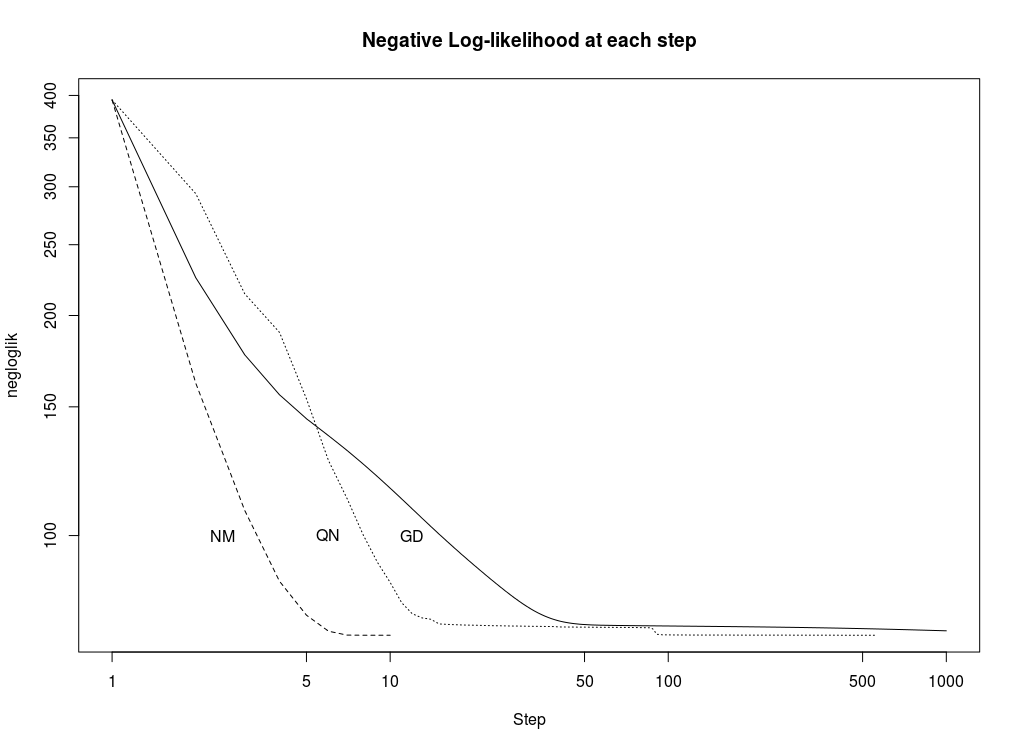
\includegraphics[width=\textwidth]{Rplot_quasi_newton.png}

The Newton method has access to the true Hessian and it's not surprising that it's able to reach convergence in 10 iterations. Quasi-Newton suffers a bit in the first few iterations because of the different $\alpha$, but it reaches pseudo convergence in few steps more, and real convergence around 500 iterations. Finally the Gradient Descent do not uses curvature information and pseudo converges in about 50 iterations.\\

\begin{tabular}{llllllll}
&\multicolumn{7}{l}{Unit:seconds} \\
&      &min      &  lq     & mean     & median   &     uq   &    max   \\
&GD & 1.68 &1.70 &1.74 &1.72 &1.78 &1.82  \\
&NM & 2.07 &2.08 &2.11 &2.09 &2.12 &2.25  \\
&QN & 7.46 &7.49 &7.57 &7.56 &7.64 &7.65  \\
&\multicolumn{7}{l}{} 
\end{tabular}

Also in this case, using more information comes with a higher running time. The benchmark shows us that Line Search in combination with the Quasi-Newton is a significantly slower algorithm compared to the other two. Surprisingly the Newton Method and the Gradient Descent are pretty close, but that can be explained by the fact that we have only 11 covariates and the Hessian calculations are still manageable.

\newpage

\subsubsection*{CODE)}

\begin{lstlisting}[basicstyle=\tiny]
library(Matrix)
library(microbenchmark)

negloglikelihood<-function(m,y,X,beta){
  total<-0
  N<-length(y)
  for(i in 1:N) total<-total+(m[i]-y[i])*t(X[i,])%*%beta+m[i]*log(1+exp(-t(X[i,])%*%beta))
  return(total)
}

gradient_negloglik<-function(m,y,X,beta){
  w<-1/(1+exp(-X%*%beta))
  S<-m*w-y
  grad<-t(X)%*%S
  return(grad)
}

gradient_descent<-function(m,y,X,beta0,stepsize,maxstepnumber,
                           accuracy_obj_fun,accuracy_beta_val){
  negloglik<-numeric(maxstepnumber)
  negloglik[1]<-negloglikelihood(m,y,X,beta0)
  gradient<-gradient_negloglik(m,y,X,beta0)
  diff_beta_val<-accuracy_beta_val+1
  diff_obj_fun<-accuracy_obj_fun+1
  i<-1
  while(!(i==maxstepnumber)&&
        ((accuracy_beta_val<diff_beta_val)||
         (accuracy_obj_fun<diff_obj_fun))){
    i<-i+1
    beta1<-beta0-stepsize*gradient
    diff_beta_val<-sum(abs(beta0-beta1))
    beta0<-beta1
    negloglik[i]<-negloglikelihood(m,y,X,beta0)
    diff_obj_fun<-negloglik[i-1]-negloglik[i]
    gradient<-gradient_negloglik(m,y,X,beta0)
  }
  return(list(betahat=beta0,negloglik=negloglik,step=i))
}

hessian_negloglik<-function(m,y,X,beta){
  w<-as.vector(1/(1+exp(-X%*%beta)))
  D<-diag(m*w*(1-w))
  hes<-t(X)%*%D%*%X
  return(hes)
}

newton_descent<-function(m,y,X,beta0,maxstepnumber,
                         accuracy_obj_fun,accuracy_beta_val){
  negloglik<-numeric(maxstepnumber)
  negloglik[1]<-negloglikelihood(m,y,X,beta0)
  gradient<-gradient_negloglik(m,y,X,beta0)
  hessian<-hessian_negloglik(m,y,X,beta0)
  diff_beta_val<-accuracy_beta_val+1
  diff_obj_fun<-accuracy_obj_fun+1
  i<-1
  while(!(i==maxstepnumber)&&
        ((accuracy_beta_val<diff_beta_val)||
         (accuracy_obj_fun<diff_obj_fun))){
    i<-i+1
    beta1<-beta0-solve(hessian,gradient)
    diff_beta_val<-sum(abs(beta0-beta1))
    beta0<-beta1
    negloglik[i]<-negloglikelihood(m,y,X,beta0)
    diff_obj_fun<-negloglik[i-1]-negloglik[i]
    gradient<-gradient_negloglik(m,y,X,beta0)
    hessian<-hessian_negloglik(m,y,X,beta0)
  }
  return(list(betahat=beta0,negloglik=negloglik,step=i))
}

line_search<-function(alpha,c1,rho,gradient,direction,m,y,X,beta){
  while(negloglikelihood(m,y,X,(beta+alpha*direction))>
        negloglikelihood(m,y,X,beta)+c1*alpha*crossprod(gradient,direction))
    alpha<-alpha*rho
  return(alpha)
}

quasi_newton<-function(mat_H0,beta0,beta1,gradient0,gradient1){
  p<-dim(mat_H0)[1]
  sk=beta1-beta0
  yk=gradient1-gradient0
  yTs<-as.numeric(crossprod(yk,sk))
  mat_H1=(diag(p)-sk%*%t(yk)/yTs)%*%mat_H0%*%(diag(p)-yk%*%t(sk)/yTs)+(sk%*%t(sk)/yTs)
  return(mat_H1)
}


line_search_quasi<-function(m,y,X,beta0,maxstepnumber,alpha,c1,rho,
                         H_start,accuracy_obj_fun,accuracy_beta_val){
  negloglik<-numeric(maxstepnumber)
  negloglik[1]<-negloglikelihood(m,y,X,beta0)
  gradient0<-gradient_negloglik(m,y,X,beta0)
  mat_H0<-H_start
  direction0<-(-mat_H0%*%gradient0)
  diff_beta_val<-accuracy_beta_val+1
  diff_obj_fun<-accuracy_obj_fun+1
  i<-1
  while(!(i==maxstepnumber)&&
        ((accuracy_beta_val<diff_beta_val)||
         (accuracy_obj_fun<diff_obj_fun))){
    i<-i+1
    stepsize<-line_search(alpha,c1,rho,gradient0,direction0,m,y,X,beta0)
    beta1<-beta0+stepsize*direction0
    gradient1<-gradient_negloglik(m,y,X,beta1)
    mat_H1<-quasi_newton(mat_H0,beta0,beta1,gradient0,gradient1)
    direction1<-(-mat_H1%*%gradient1)
    negloglik[i]<-negloglikelihood(m,y,X,beta1)
    diff_obj_fun<-negloglik[i-1]-negloglik[i]
    diff_beta_val<-sum(abs(beta0-beta1))
    beta0<-beta1
    gradient0<-gradient1
    direction0<-direction1
  }
  return(list(betahat=beta0,negloglik=negloglik,step=i))
}

data_wdbc<-read.csv("./wdbc.csv", header=FALSE)
X<-as.matrix(cbind(rep(1,569),scale(data_wdbc[,3:12])))
y<-data_wdbc[,2]
y<-as.numeric(y=="M")
m<-rep(1,569)

beta0<-rep(0,11)
stepsize<-0.02
alpha<-0.06
c1<-0.0001
rho<-2/3
H_start<-diag(11)
maxstepnumber<-1000
accuracy_obj_fun<-0.001
accuracy_beta_val<-0.001

result_grad_desc<-gradient_descent(m,y,X,beta0,stepsize,maxstepnumber,
                                   accuracy_obj_fun,accuracy_beta_val)
result_newton_desc<-newton_descent(m,y,X,beta0,maxstepnumber,
                                   accuracy_obj_fun,accuracy_beta_val)
result_ls_quasi<-line_search_quasi(m,y,X,beta0,maxstepnumber,
                                   alpha,c1,rho,H_start,
                                   accuracy_obj_fun,accuracy_beta_val)

result_grad_desc$betahat
result_newton_desc$betahat
result_ls_quasi$betahat

plot(result_grad_desc$negloglik[1:result_grad_desc$step],
     main = "Negative Log-likelihood at each step",
     xlab="Step",ylab="negloglik",type="l",log="xy")
points(result_newton_desc$negloglik[1:result_newton_desc$step],
       type="l",lty=2)
points(result_ls_quasi$negloglik[1:result_ls_quasi$step],
       type="l",lty=3)
text(3, 100, "NM")
text(7, 100, "QN")
text(12, 100, "GD")

maxstepnumber<-100
accuracy_obj_fun<-0
accuracy_beta_val<-0
comparison<-microbenchmark(times=10,
result_grad_desc<-gradient_descent(m,y,X,beta0,stepsize,maxstepnumber,
                                   accuracy_obj_fun,accuracy_beta_val),
result_newton_desc<-newton_descent(m,y,X,beta0,maxstepnumber,
                                   accuracy_obj_fun,accuracy_beta_val),
result_ls_quasi<-line_search_quasi(m,y,X,beta0,maxstepnumber,
                                   alpha,c1,rho,H_start,
                                   accuracy_obj_fun,accuracy_beta_val))
comparison
\end{lstlisting}

\end{document}